\section{Comparison Metrics}

In this study response spectra is the most important factor to choose the best model. As we discussed the equivalent linear method is a linear process, therefore, the final displacement will not be accurate specially when we have a permanent displacement. Therefore, acceleration and response spectra would be the best options. A simple method to compute the response spectra residuals is subtracting two data and divide them by one of them. 


\begin{equation}
Residual_{Sa} = mean[\frac{Sa_{nonlinear} - Sa_{equivalent linear}}{Sa_{nonlinear}}],
\end{equation}

According to this equation, if nonlinear simulation results is much higher than equivalent linear, then the residual will be one, however, if it is much lower, the residual will be a negative number. The problem with this method is its weakness in representing higher residuals in more than 1 for the positive residuals.  Other approaches are mentioned in the literature to compare the response spectra of two waveform. \citet{Anderson_2004_Proc} uses,

\begin{equation}
S_{sa} = mean[S(SA_1(f_j),SA_2(fj))],
\end{equation}

where the average is over all frequencies at which SA is computed in the frequency band being considered. And $S $ defined as,

\begin{equation}
	S( p_1, p_2) = 10 exp \{ - [ \frac{(p_1 - p_2)}{ \min( p_1, p_2 ) }]^2 \},
\end{equation}

The equation, which is used for GOF score, put the scores from comfortable range of values (0-10) regarding the poorest fit and excellent fit. This is a very good scale, however, it can not represent which simulation had a higher values. Because the results are always positive.  \citet{Assimaki2008quantifying} used cumulative normalized error between observation and prediction:

\begin{equation}
e_{SA}=\frac{1}{n}\sqrt{\sum_{i=1}^{n}[\frac{SA_o(T_i)-SA_p(T_i)}{SA_o(T_i)}]^2}
\end{equation}

This metric also represents positive residual values. 

\citet{Assimaki2012} and \citet{Carlton2016comparison} used the following equation to measure of misfit between two $SA$:

\begin{equation}
e_{SA}^{non}=\mu(e_{SAi})=\mu(log(\frac{SA_{i}^{non}}{SA_{i}^{eq}}))
\end{equation}

This metric can represent a good variation of residuals and does not saturate. Also positive residuals represent higher values for nonlinear and negative values represent higher values for equivalent linear. Fig.~\ref{fig:response_spectra_sensitivity} shows the relationship between these metrics. In this study we use logarithmic residuals. 


\begin{figure}
    \centering
    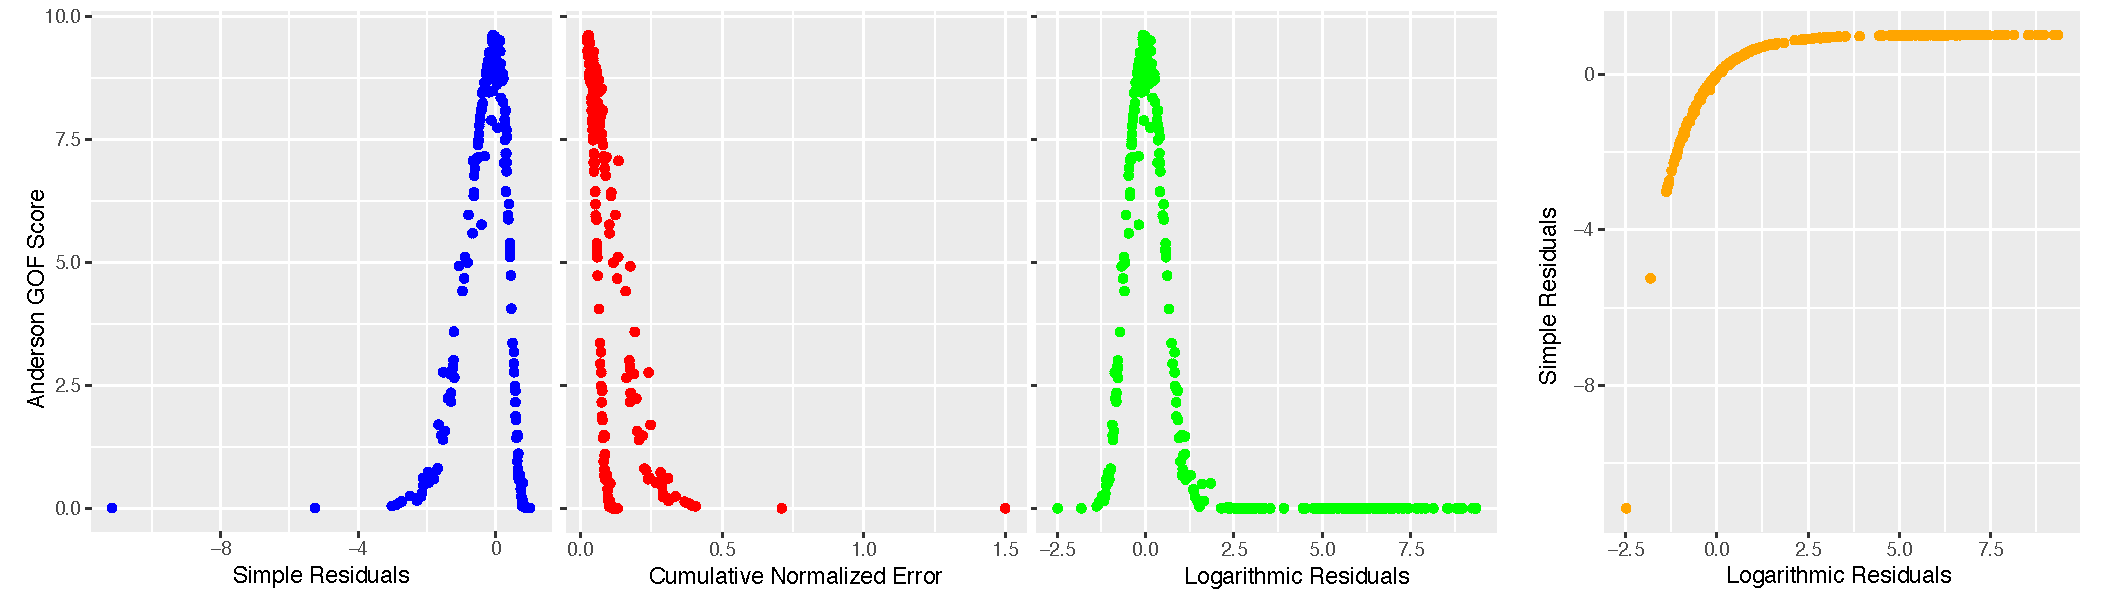
\includegraphics[width=\textwidth]{figures/pdf/response_spectra_sensitivity.pdf}
    \caption{}
    \label{fig:response_spectra_sensitivity}
\end{figure}


